
\chapter{Implementation}

\section{Operation}
Text editing can be realized with only two operations. 
 - Insert
 - Delete
 - Split

All operations have some equivalent properties. They must provide a function called \texttt{inverse()} that returns the inverse operation, a . 

They are represented by the Operation Interface.
 
\subsection{Operation Hierarchy}
\begin{figure}[H]
\centering
\includegraphics[height=5.74cm,width=11.59cm]{../../images/algo-impl/operation_classdiagram.eps}
\caption{Operation Hierarchy}
\label{Operation Hierarchy}
\end{figure}

\subsection{InsertOperation}


\subsection{DeleteOperation}
\subsection{SplitOperation}
\label{Split_Operation}
  - no operation
  - wrapper to handle special cases -> \ref{Delete_Insert}


\newpage
\section{Request}
\begin{figure}[H]
\centering
\includegraphics[height=6.87cm,width=12.09cm]{../../images/algo-impl/request_classdiagram.eps}
\caption{Request Class Diagram}
\label{Request Class Diagram}
\end{figure}


\newpage
\section{GOTO Transformation Functions}

\subsection{Overview}
The GOTO (generic operation transformation optimized) transformation functions are designed to work with strings. The advantage is that less transformations are needed when a string has been inserted into a text. To understand the exigence of transformation functions see \emph{Report Evaluation Algorithms}.

The inclusion transformation functions are used to check the influence of a given operation B to another operation A. If so, the operation A will be transformed into operation A'. To transform an operation means to adapt position and text of the operation. In the majority of cases this is a very simple process. But sometimes it is necessary to extract a text fragment or to split up an operation in two parts. For more details about splitting operations into two parts see \ref{Split_Operation}.

All possible transformations \emph{cases} with two insert/delete operations are represented by figure \ref{Transformation Overview} and explained in the following sections:
\begin{figure}[H]
\centering
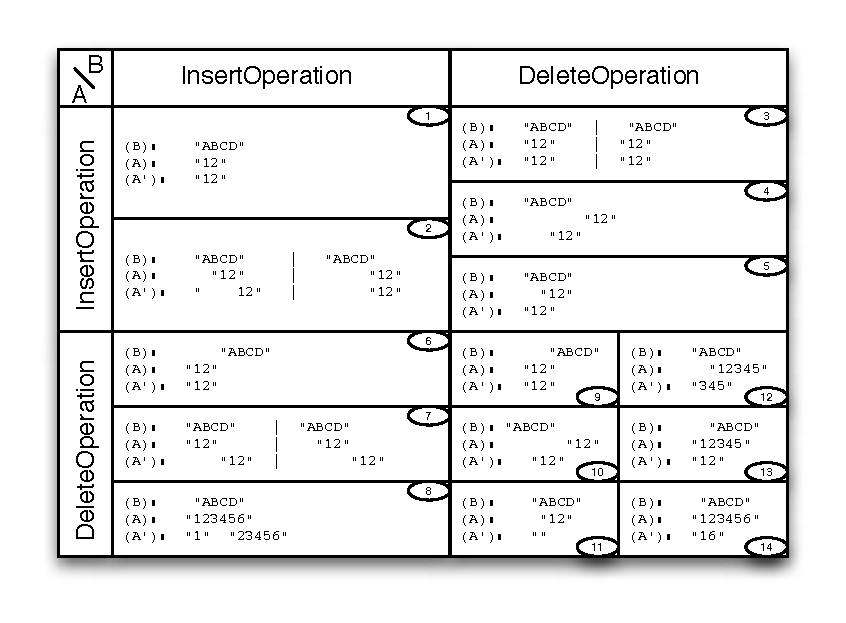
\includegraphics[height=9.98cm,width=13.75cm]{../../images/algo-impl/transform_overview.eps}
\caption{Transformation Overview}
\label{Transformation Overview}
\end{figure}

\subsection{Insert/Insert}
\begin{itemize}
\item \textbf{Case 1:}
Operation A starts before or at the same position as operation B. Sometimes some special handling is necessary. See \emph{Special Case} in section \ref{Special_Case} for detailed information about that.
\item \textbf{Case 2:}
Operation A starts in or behind operation B. Index of operation A' must be increased by the length of the text of operation B.
\item \textbf{Special case:}
\label{Special_Case}
It can occur that two insert operations (for example \texttt{Ins(1,'a')} and \texttt{Ins(1,'b')}) have the same position. How should the correct transformation looks like (has the insertion of 'a' to be before or after 'b')? This is an undecidable problem. Therefore some extra rules must be defined. The first approach to solve this problem is by preferring the operation with the lower ascii value. With this method the final text would be \texttt{ab}. The following figure demonstrates that this solution can violate the user intention:
\begin{figure}[H]
\centering
%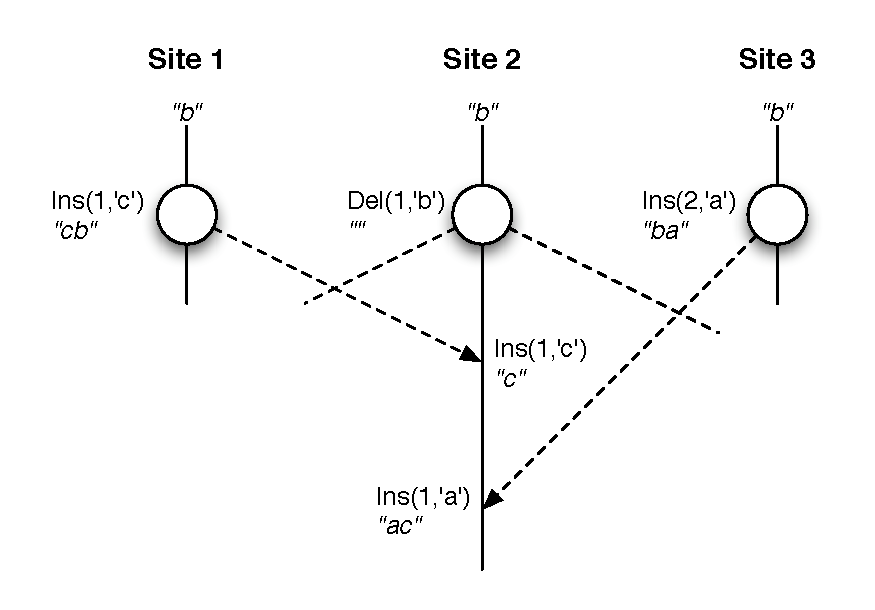
\includegraphics[height=9.77cm,width=14.25cm]{../../images/algo-impl/transform_ins_ins_charpos.eps}
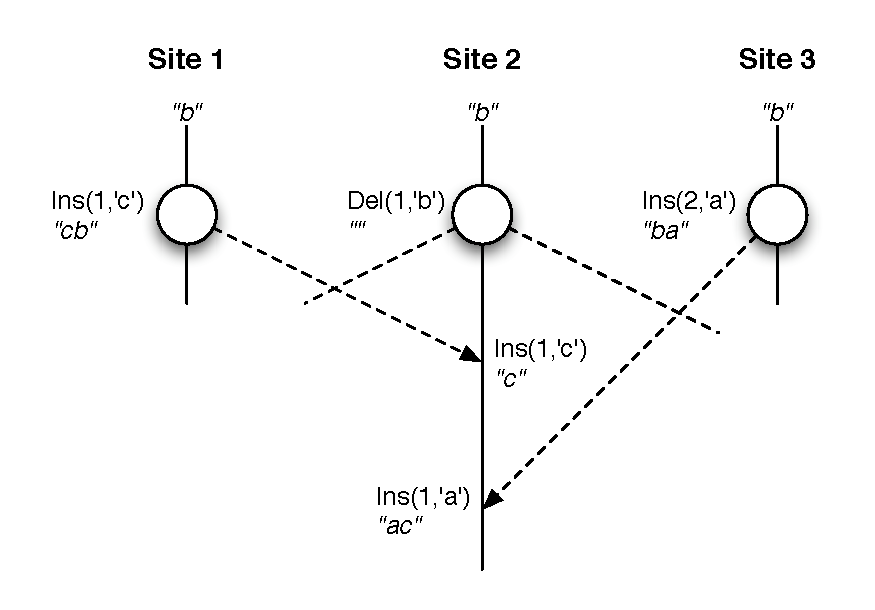
\includegraphics[height=4.63cm,width=7.12cm]{../../images/algo-impl/transform_ins_ins_charpos.eps}
\caption{Insert based on character ord}
\label{Insert based on character ord}
\end{figure}
The scenario described in figure \ref{Insert based on character ord} demonstrates an editing session with 3 users (sites). Each site is generating a request at the same time. For simpleness only the process flow at site 2 is shown. The initial document state was \texttt{b}. After applying the own operation (\texttt{Del(1,'b')}) then document is empty. Now there arrives two operation. First the operation \texttt{Ins(1,'c')} from site 1 and then \texttt{Ins(2,'a')} from site 3 which will be transformed into \texttt{Ins(1,'a')} because the delete operation has an effect on it. The two operations (\texttt{Ins(1,'a')} and \texttt{Ins(1,'b')}) left and the problem described in the previous paragraph occures.

The second approach is working with some exrta informations. If an operation has been generated the original position is saved too. Adapted to the scenario in figure \ref{Insert based on character ord} the insert operation of site 1 would looks like \texttt{Ins(1,'a',1)}. Similar to the insert operation of site 1 the insert operation of site 3 looks like \texttt{Ins(2,'b',2)}. The added third parameter representing the original position. At the beginning the position and the original position have the same value. The differece of the two positions is shown after a transfomation. Unlike the position (first parameter) the original position will never be transformed/changed and remains with the original value.

Now site 1 sends the request \texttt{Ins(1,'c',1)} to site 2. After site 2 received the request, site 3 sends the request \texttt{Ins(2,'a',2)}. On site 2 this request will be first transformed with \texttt{Del(1,'b')} into \texttt{Ins(1,'a',2)}. This is necessary because while site 3 was generating the request, site 2 deleted the character \texttt{b}. After this transformation the new request have to be transformed with the request from site 1. This transformation would looks like \texttt{transform( Ins(1,'a','2'), Ins(1,'c',1) )} which means that the effect from the operation \texttt{Ins(1,'c',1)}) will be included into operation \texttt{Ins(1,'a',2)}. The problem to solve now is the same as before, but with the extra information its not longer infeasible. After detecting that the two operations have the same position the transformation function compares the original positions. With this solution the \texttt{c} will be inserted before the \texttt{a} and the user intention is preserved.

Figure \ref{Insert based on original positions} shows that even with using original positions another problem can occur:
\begin{figure}[H]
\centering
%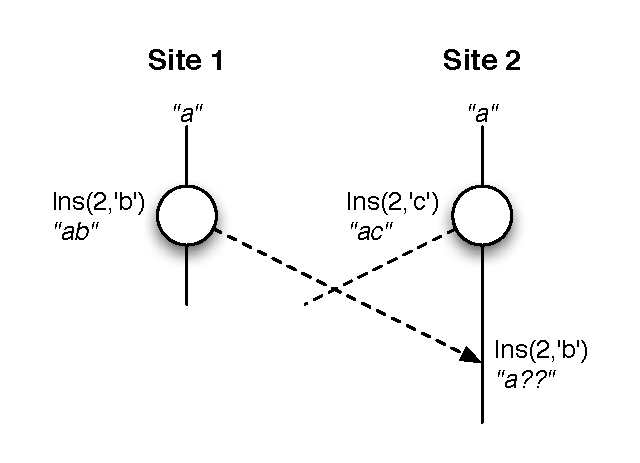
\includegraphics[height=7.26cm,width=10.26cm]{../../images/algo-impl/transform_ins_ins_origpos.eps}
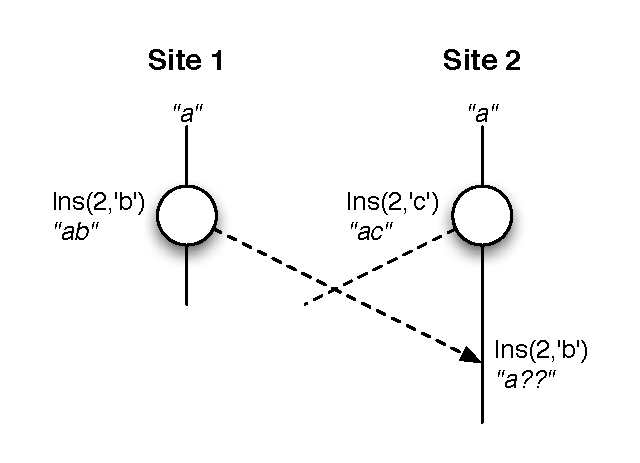
\includegraphics[height=3.63cm,width=5.13cm]{../../images/algo-impl/transform_ins_ins_origpos.eps}
\caption{Insert based on original positions}
\label{Insert based on original positions}
\end{figure}
At the same time each site generates an insert operation with the same position. The insert operation from site 1 looks like \texttt{Ins(2,'b',2)} and the operation from site 2 is \texttt{Ins(2,'c',2)}. When site 2 receives the request from site 1 the operations have to be tranformed (\texttt{transform( Ins(2,'b',2) , Ins(2,'c',2) )}). The transform function will detect that the two operations have the same position and will check the original positions. Unfortunately the original positions have the same values. Therefore the approach to solve this problem by using original positions will fail too.

This problem can only be eliminated by privileging one operation. But which operation should be preferred? And how to guarantee that on all sites this will be the same operation? One possible solution would be to use the site id's (e.g. site 1 is always privileged against site 2 and site 3, site 2 is only to site 3). Especially when using this tranformation functions with the jupiter algoritm always the operation generated on the server part can be privileged.
\end{itemize}

\subsection{Insert/Delete}
\begin{itemize}
\item \textbf{Case 3:}
Operation A starts before or at the same position as operation B. Nothing has to be transformed.
\item \textbf{Case 4:}
Operation A starts after operation B. Index of operation A' must be reduced by the length of the text of operation B.
\item \textbf{Case 5:}
Operation A starts in operation B. Index of operation A' must be the index of operation B.
\end{itemize}

\subsection{Delete/Insert}
\begin{itemize}
\item \textbf{Case 6:}
Operation A is completly before operation B. Nothing has to be transformed.
\item \textbf{Case 7:}
Operation A starts before or at the same position as operation B. Index of operation A' must be increased by the length of the text of operation B.
\item \textbf{Case 8:}
Operation B is in the range of operation A. Operation A' must be splitted into two delete operations. For more details about this process see \cite{Split_Operation}.
\end{itemize}

\subsection{Delete/Delete}
\begin{itemize}
\item \textbf{Case 9:}
Operation A is completly before operation B. Nothing has to be transformed.
\item \textbf{Case 10:}
Operation A starts at the end or after operation B. Index of operation A' must be reduced by the length of the text of operation B.
\item \textbf{Case 11:}
Operation A and operation B are overlapping. Operation B starts before or at the same position as operation A and ends after or at the same position as operation A. Content of operation A has been already deleted by operation B. Nothing has to be deleted by operation A. A' is called a noop (no-operation).
\item \textbf{Case 12:}
Operation A and operation B are overlapping. Operation B starts before or at the same position as operation A and ends before operation A. The overlapping part of the two operations has been deleted by operation B. Operation A' has to delete only the remaining text (text after the overlapping text of the two operations).
\item \textbf{Case 13:}
Operation A and operation B are overlapping. Operation B starts after operation A and ends after or at the same position as operation A. The overlapping part of the two operations has been deleted by operation B. Operation A' has to delete the remaining text (text before the overlapping text of the two operations).
\item \textbf{Case 14:}
Operation A and operation B are overlapping. Operation B is fully in operation A. The overlapping part of the two operations has been deleted by operation B. Operation A' has to delete the remaining text (text before and after the overlapping text of the two operations).
\end{itemize}



\section{Client}


\section{Server}


\section{Undo/Redo}



\section{Tests}
Testing the algorithm implementation was considered a very high priority. Without a correctly working algorithm, it will be difficult or even impossible to create a collaborative text-editor. Because of the significance of this algorithm we invested a lot of time to test it.

\subsection{Testframework}
In the literature about operational transformation, so called puzzles are omnipresent. These puzzles are exact specification of the order of events, like the generation of a request or the reception of a request. We were soon convinced that in order to test our algorithm it would be possible to have a testframework that accepts such a puzzle (called scenario) as input and replays the sequence of events on a set of algorithms. To find out more about this testframework, see the document 'Report Implementation Testframework'.

\subsection{Test Cases}
We gathered many test cases form publications about operational transformation algorithms. The puzzles presented in these papers often represent particularly tricky issues that other algorithms failed to resolve. Here is a list of test cases that were taken from papers:

% TODO: insert all test cases that were taken from papers
\begin{itemize}
 \item 
 \item 
 \item 
\end{itemize}

Our algorithm is capable of solving these complex puzzles. This is a step in the right direction, but that alone is not enough. So we devised additional test cases that cover trivial as well as complex scenarios.

\subsection{JUnit Tests}
It is one of our goals to have a good test coverage with \emph{JUnit} tests.
